\section{Mathematical Formula}
In this section, Kualala is going to use latex to write some mathematical formulas and math symbols.

\subsection{Mathematical Formula-ex.1-symbol example}
Here is the Greek alphabet below, both lowercase and capital.
\begin{figure}[H]
    \centering
    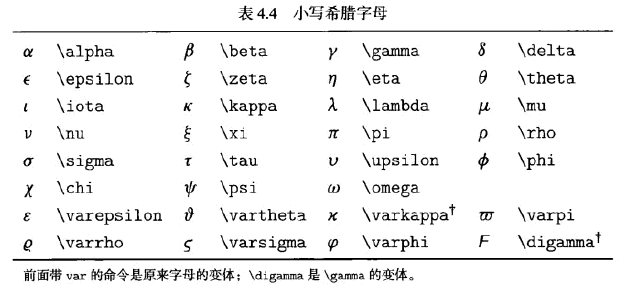
\includegraphics[scale=0.6]{Test/Test-formula/Greek-lowercase.png}
    \caption{Greek alphabet-lowercase.}
    \label{fig:Greek alphabet-lowercase}
\end{figure}

\begin{figure}[H]
    \centering
    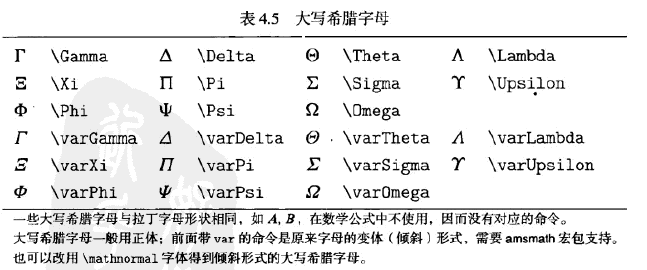
\includegraphics[scale=0.6]{Test/Test-formula/Greek-capital.png}
    \caption{Greek alphabet-capital.}
    \label{fig:Greek alphabet-capital}
\end{figure}

Here is some normal mathematical symbols.
\begin{figure}[H]
    \centering
    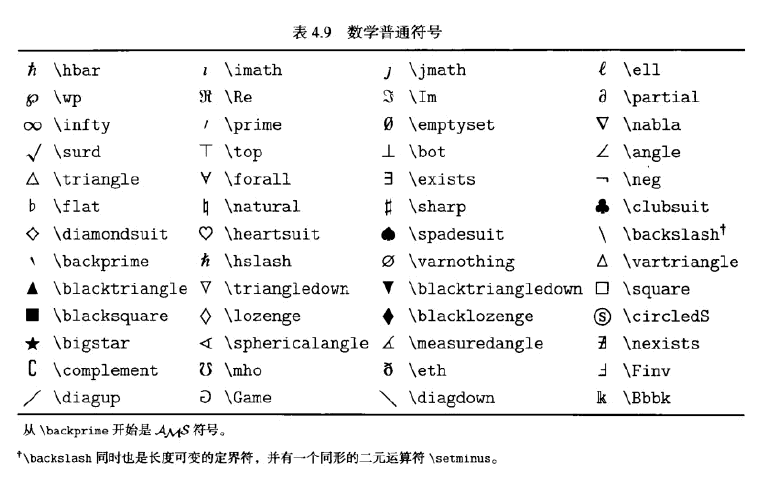
\includegraphics[scale=0.6]{Test/Test-formula/Normal symbols.png}
    \caption{Normal mathematical symbols.}
    \label{fig:Normal mathematical symbols.}
\end{figure}

Here is some relation symbol.
\begin{figure}[H]
    \centering
    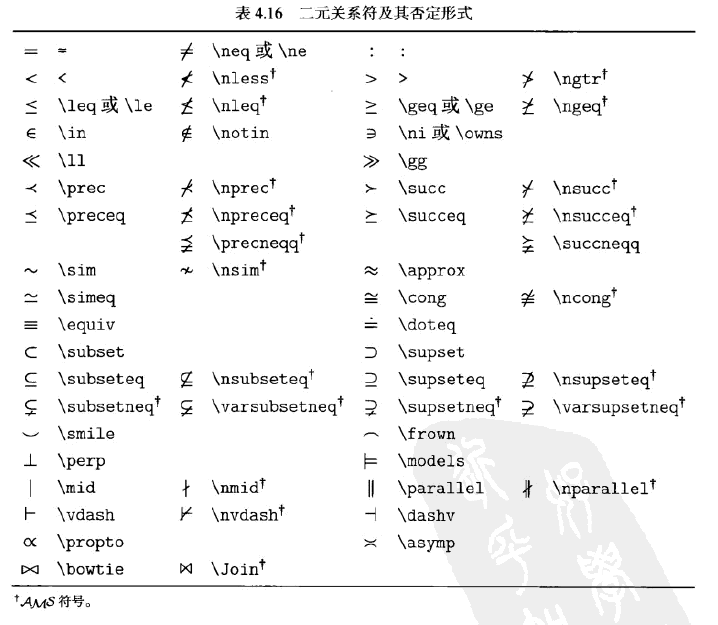
\includegraphics[scale=0.6]{Test/Test-formula/Relation symbols.png}
    \caption{Relation symbol.}
    \label{fig:Relation symbol}
\end{figure}

Here is other mathematical symbols.

$\dag$  \qquad  $\S$    \qquad  $\checkmark$

%%二项式系数
binomial coefficient:   \qquad
$\binom{2n}{n+1}$

\subsection{Mathematical Formula-ex.2-formula example}

$A_m^n$ \qquad  $A_m{}^n$   %%改变上标位置

$A_{ij} = 2^{i+j}$

$\overset{*}{X}$    \qquad
$\underset{*}{X}$   \qquad
$\overset{*}{\underset{\dag}{X}}$

Here we use tool to write a formula and give number to it.

Like for a sequence, see in Formula \ref{foumula:sequence}.

\begin{equation}
    K_{N_i} = K_{2^i} = 2^{N_i} = 2^{2^i}
    \label{foumula:sequence}
\end{equation}

Here are some examples below.

$3^{3^{3^{\cdot^{\cdot^{\cdot^3}}}}}$

$\angle A = 90^{\circ}$

%%sigma求和
$\max_n f(n) = \sum_{i=0}^n A_i$    \qquad
There is another writing way (or two more lines)
\[
    \max_n f(n) = \sum_{i=0}^n A_i
\]

%%sigma求和下标有两行
\[
    \sum_{\substack{0<i<n \\ 0<j<i}} A_{ij}
\]

%%prod求积
\[
    \sum_{i=0}^n A_i = \prod_{k=1}^m B_k
\]

%%积分
\[
    \int_0^1 f(t) \dif t = \iint_D g(x,y) \dif x \dif y
\]

%%求偏导
%%\left和\right可以转换为开符号和闭符号，并且自动调节大小
\[
    \partial_x \partial_y \left[
    \frac{1}{2} \left(x^2+y^2 \right)^2+xy
    \right]
\]

%%上下划线
$\overline{a+b} = \overline{a} + \overline{b}$, 
$\underline a = (a_0, a_1, a_2, \dots)$

%%上下箭头和花括号
$\overleftarrow{a+b}$, 
$\overleftrightarrow{a+b}$, 
$\overbrace{a+b+c}^{\text{$n+1$}} = \underbrace{1+2+3}$

\subsection{Mathematical Formula-ex.3-matrices}
Here are three kinds of matrices below.
%%圆括号矩阵
\[
    A = \begin{pmatrix}
            a_{11} & a_{12} & a_{13}    \\
            0 & a_{22} & a_{23}    \\
            0 & 0 & a_{33}
        \end{pmatrix}_{n\times n}
\]

%%方括号矩阵带矩阵大小
\[
    A = \begin{bmatrix}
            a_{11} & \dots & a_{in} \\
              & \ddots & \vdots  \\
            0 &  & a_{nn}
        \end{bmatrix}_{n\times n}
\]

%%矩阵元素位数不同对称，需要mathtools宏包
\[
    A = \begin{pmatrix*}[r]
            10 & -10 \\ -20 & 3
        \end{pmatrix*}_{2\times 2}
\]

\subsection{Mathematical Formula-ex.4-formulas more than one row}
Here is an example.
%%多行公式
\begin{gather}  %%编号环境
    a+b = b+a   \\
    ab = ba
\end{gather}

Here is another example.
\begin{gather*} %%不编号环境
    3+5 = 5+3 = 8   \\
    3\times 5 = 5\times 3
\end{gather*}

\begin{gather}
    3^2 + 4^2 = 5^2 \notag \\ %%手动不编号
    5^2 + 12^2 = 13^2 \notag \\ %%手动不编号
    a^2 + b^2 = c^2
\end{gather}    

\begin{align}
    x &= t + \cos t + 1 \\
    y &= 2 \sin t
\end{align}

\begin{align*}
    x &=t  & x &= \cos t    & x & = t \\
    y &=2t & y &= \sin(t+1) & y & = \sin t
\end{align*}

\begin{equation}
    \label{eq:dakuohao}
    D(x) = \begin{cases}
    1, & \text{if } x \in \mathbb{Q}; \\
    0, & \text{if } x \in \mathbb{R}\setminus\mathbb{Q}.
    \end{cases}
\end{equation}In this section, Kualala is going to use latex to write some mathematical formulas and math symbols.

